\documentclass[12pt]{article}
\usepackage{indentfirst}
\usepackage{graphicx}
\usepackage{textcomp}
\usepackage{siunitx}
\usepackage{subcaption}
\usepackage{amsmath}
\usepackage{setspace}
\usepackage{url}
\usepackage[a4paper,margin=2.54cm]{geometry}

\title{Computer Science II \\Project 2: Comparison of Sorting Algorithms}
\author{TAERAKUL Janat, \#19B60096}
\date{January 31, 2020}
\renewcommand{\UrlFont}{\small\tt}

\begin{document}

% \onehalfspacing
% \doublespacing

\maketitle

\section{Sorting}\label{sec:instr}

	In computer science, sorting is one of fundamental algorithms. It simply puts a set of data in a certain order. Efficient sorting can help optimizing other algorithms such as searching ($O(logn)$) and merging ($O(n)$).
	
	\begin{figure}[ht]
		\centering
		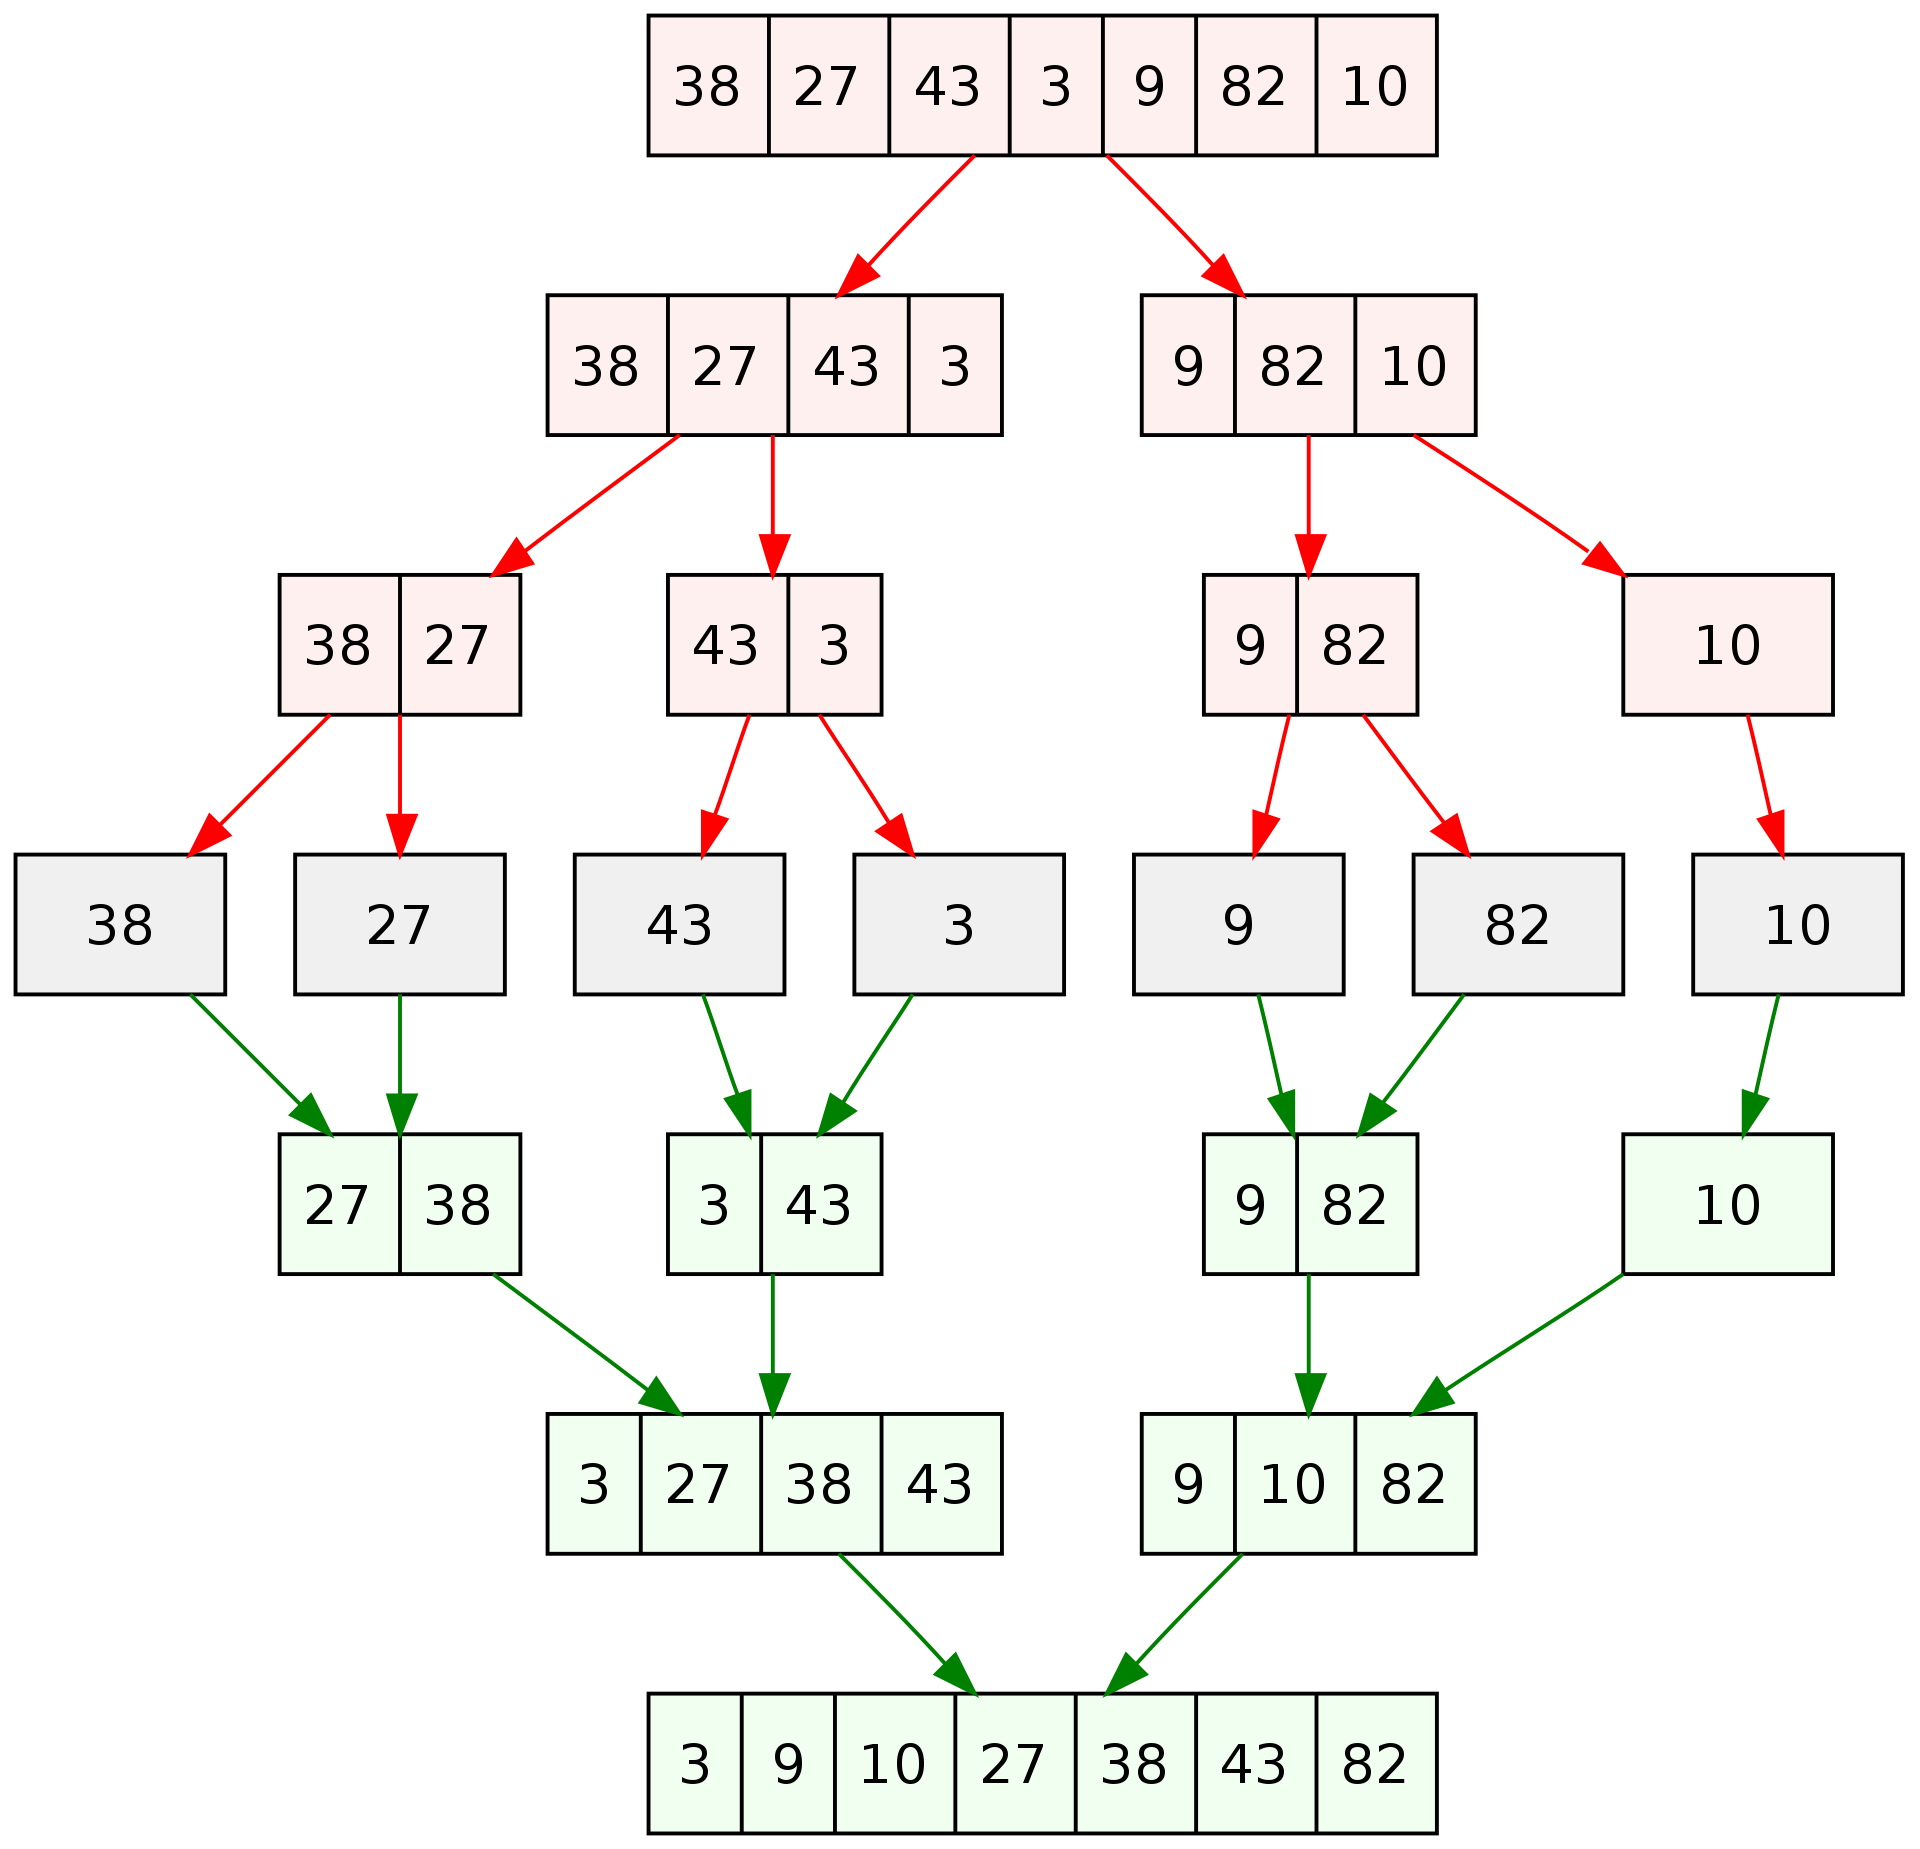
\includegraphics[height=5cm]{Merge_sort_algorithm_diagram.png}
	\end{figure}


\section{Algorithms}\label{sec:how}
	
	\subsection{Merge Sort}
	
	\textbf{Merge Sort} is similar to the method called Divide-and-conquer. It divides an input array into two sub array, sort them and using benefit from sorted array to merge two array in linear time ($O(n)$). The sorting step, it sorts the array by calling itself (Recursion function). The base case of recursion is when the size of the array is one (the array of one number is a sorted array), it returns the input array.
	
	\begin{verbatim}
	def sort(array):
	    n = len(array)
	    if n < 2:                   // when the size of array is one,
	        return array            // it returns the input array
	    mid = n // 2
	    left = sort(array[:mid])    // Sort the left array
	    right = sort(array[mid:])   // Sort the right array
	    return merge(left, right)   // Return the merged array
	\end{verbatim}
	
	\subsection{Selection Sort}
	
	\textbf{Selection Sort} is an $O(n^2)$ sorting algorithm. The main concept of the algorithm is to find the least element in an array and swap it with the first element of the array. Every time the least element is selected, the unsorted array is reduced from $n$ elments to $n-1$. The process has to be run for n times, therefor, the time complexity is $O(n^2)$
	
	\begin{verbatim}
	def sort_inplace(array):
	    n = len(array)
	    for i in range(n-1):
	        minidx = i
	        for j in range(i, n):
	            if array[minidx] > array[j]:
	                minidx = j        // Find the least element in the array
	        // Swap the least element and the first element
	        swap(array, i, minidx)
	    return array
	\end{verbatim}
	
	\subsection{Bubble Sort}
	
	\textbf{Bubble sort} is similar to the bubble that float up. Its method is to check the $i^{th}$ element and the $(i+1)^{th}$ element of the input array. If the $i^{th}$ element is greater, then swap them. The loop runs from $0$ to $n-1$. Every times the loop complete, the greatest element in array will float to the right of the array (The loop has to be run for $n$ times). Therefore, the complexity is $O(n^2)$
	
	\begin{verbatim}
	def sort_inplace(array):
	    n = len(array)
	    for i in range(n-1):
	        for j in range(n-i-1):
	            if array[j] > array[j+1]:
	                // Swap the greater element to the right
	                swap(array, j, j+1)
	    return array
	\end{verbatim}
	
	\subsection{Heap Sort}
	
	\begin{figure}[ht]
		\centering
		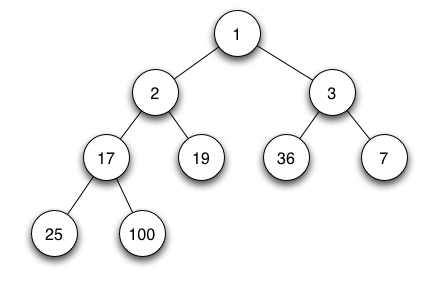
\includegraphics[height=5cm]{Min-heap.png}
		\caption{Min Heap}
		\label{fig:minHeap}
	\end{figure}
	
	\textbf{Heap sort} uses the data structure called Min Heap (Figure \ref{fig:minHeap}). The heap \textbf{always} has the least element on the top. Each node has two children, both of them has to be more then the parent. The heap always maintain its property. I implemented heapify (Initiate the array into a min heap ($O(n)$)) and pop (Remove the top element of the heap and return its value (min value) ($O(logn)$)). The sorting part is just simply heapify the array and the pop the heap until the last element comes out which cost $O(Nlogn)$
	
\newpage
\section{Comparison of Sorting Algorithms}

	\begin{figure}[ht]
		\centering
		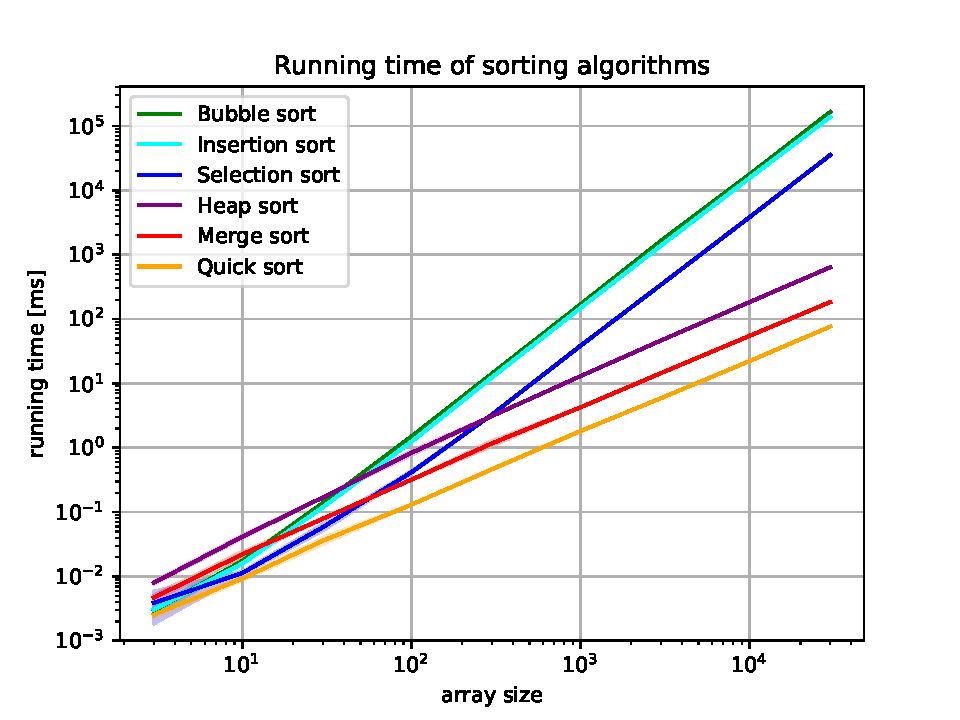
\includegraphics[height=8cm]{sort_comparison.pdf}
		\caption{Comparison of Sorting Algorithms}
		\label{fig:sortComp}
	\end{figure}
	
	The graph show the rate of growth of each function. From the graph,  bubble sort, insertion sort, selection sort are $O(n^2)$ and merge sort, quick sort, and heap sort are $O(nlogn)$. The difference in each sorts are vrarie due to the time constant 
	


\end{document}